
\chapter{算法实现}

\section{图像预处理}

受光照条件和噪声等因素的影响,图像的质量不佳,不能直接用于数字识别。需要进行预处理,改善图像质量,从而更容易识别数字。本文采用的预处理方法先后有\emph{灰度化},\emph{高斯滤波}和\emph{直方图均衡}。

\subsection{灰度化}



摄像头采集的图像是彩色图像,如图\ref{fig:src}所示。由于待识别的数字在右上角,所以只需截取右上部分做后续处理,如图\ref{fig:rgb}所示。首先将彩色图像转换成灰度图像。这样做的原因是:
\begin{asparaenum}[(1)]
\item 灰度图像只有一个分量,比三分量的彩色图像更易处理;
\item 本文识别的数字边框为黑底白字,边框内绝大部分像素都是黑白颜色,灰度化后颜色基本没有变化。
\end{asparaenum}

本文使用加权平均法求出灰度图像,公式为$I=0.114R+0.587G+0.299B$。灰度图像如\ref{fig:gray}所示。
\begin{figure}[h]
  \centering
  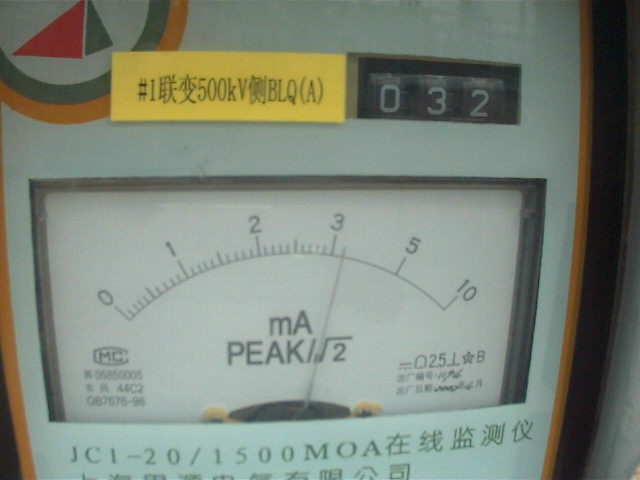
\includegraphics[scale=0.5]{src.png}
  \caption{原始图像}
  \label{fig:src}
\end{figure}
\begin{figure}[h]
  \centering
  \subfloat[彩色图像]{\label{fig:rgb}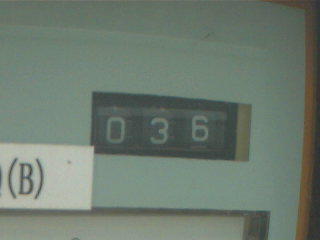
\includegraphics[scale=0.5]{rgb.png}}\hspace{1in}
  \subfloat[灰度图像]{\label{fig:gray}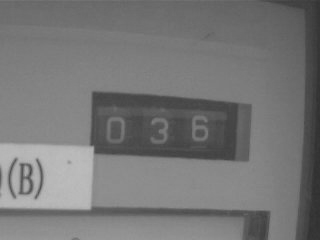
\includegraphics[scale=0.5]{gray.png}}
  \caption{灰度化}
\end{figure}

\subsection{高斯滤波}


灰度图像含有较多噪声,不利于提取目标,需要用图像平滑的方法减少噪声。观察发现,待处理图像的噪声以盐椒噪声为主,因此选用高斯滤波进行平滑滤波。在调用OpenCV的高斯滤波函数时,要指定高斯滤波模板的长宽,$\sigma$值和边界扩充类型。一般情况下,只需使用长宽相等的高斯滤波模板。模板尺寸越大,平滑的效果越好,但图像的边缘也越模糊。综合以上情况,将长和宽均设置为3。$\sigma$值的设定也有一定的要求。高斯函数在半径为$2\sigma$范围内的积分为0.95,故绝大部分权值集中在这个领域内。为了最大限度地发挥高斯滤波的效果,需要保证模板能覆盖这个邻域,故选择$\sigma=\frac{2}{3}$。边界扩充类型指将高斯滤波模板中心与图像边界重合,模板覆盖的部分像素超出图像边界时,这部分像素值的计算方式。一般的做法是将边界内的像素值复制到边界外。高斯滤波的效果如\ref{fig:gauss}所示。
\begin{figure}[h]
  \centering
  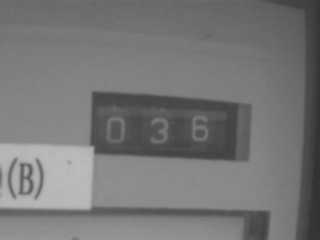
\includegraphics[scale=0.5]{gaussian.png}
  \caption{高斯滤波}
  \label{fig:gauss}
\end{figure}

\subsection{直方图均衡}


由于不同时间内光照条件不同,不同时间采集的图像的整体亮度不同。例如日光微弱时图像整体偏暗,日光强烈时图像整体偏亮。偏暗和偏亮的图像对比度不高,不利于识别。因此,采用直方图均衡化的方法增强图像的动态范围,从而达到增强图像整体对比度的效果。实验发现,在进行直方图均衡化前,需要进行图像平滑。这是因为直方图均衡对图像的所有像素的灰度不加选择地加以扩充,因此噪声的灰度也被扩充,使原本灰度相近的区域灰度差距加大,对图像分割造成不利影响。

比较均衡化前的直方图\ref{fig:histsrc}和均衡化后的直方图\ref{fig:histequal}分别是均衡化前和均衡化后的直方图,可以发现均衡化后的直方图比均衡化前的直方图具有更宽的动态范围,每个灰度级上有大致相等的像素数。
\begin{figure}[h]
  \centering
  \subfloat[均衡化前的直方图]{\label{fig:histsrc}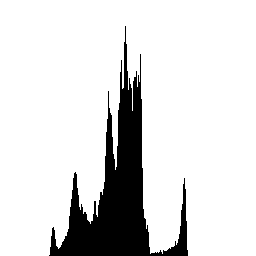
\includegraphics[scale=0.5]{histsrc.png}}
  \subfloat[均衡化后的直方图]{\label{fig:histequal}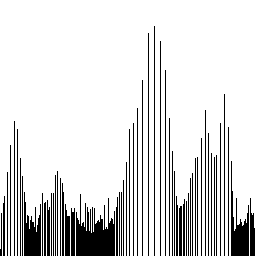
\includegraphics[scale=0.5]{histequal.png}}
  \caption{均衡化前后的直方图}
\end{figure}
直方图均衡化后的图像如图\ref{fig:equal}所示。经直方图均衡化后,不同时间的图像灰度分布大致相同,对于图像分割和识别是十分有益的。
\begin{figure}[h]
  \centering
  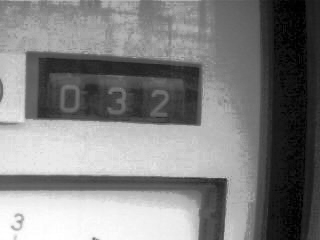
\includegraphics[scale=0.5]{equal.png}
  \caption{直方图均衡化}
  \label{fig:equal}
\end{figure}



\section{数字边框定位}

数字边框定位是电表读数识别的一个关键环节,也是较难的环节。数字边框内的数字是待识别的目标,数字边框外的图像则为无用信息。直接从原图中提取数字,难度大,准确率低。因此,应首先找出数字边框,去除无用的部分。观察图\ref{fig:equal}发现,数字边框周围有一些干扰区域,如右侧的电表边框和下侧的指针边框颜色灰度和数字边框的背景类似。这些干扰区域增加了分割的难度。

\subsection{二值化}

数字边框定位的第一步是二值化,即将原图分割为目标区域和背景区域,将目标区域的灰度设为255,背景区域的灰度设为0。观察图像发现,图像的各个区域内灰度差别较小,区域间灰度差别较大,适合用阈值法分割。阈值分割的关键是找到阈值。由于本文的灰度图像由大片的黑色和白色区域组成,可以使用Otsu算法分割阈值,

由式\eqref{eq:otsu}可得,Otsu算法需要对每个可能的灰度$t$计算$q_1(t),q_2(t),\mu_1(t),\mu_2(t)$四项。如果直接根据式\eqref{eq:musig}计算这四项,计算过程复杂而低效。为了简化计算,可以将式\eqref{eq:musig}改写成递推公式:
\begin{equation}
  \label{eq:recursive}
  \begin{aligned}
    q_t(t+1) &=q_1(t)+P(t+1)\\
    q_2(t+1) &=1-q_1(t) \\
    \mu_1(t+1) &=\frac{\mu_1(t)q_1(t)+(t+1)q_1(t+1)}{q_1(t+1)} \\
    \mu_2(t+1) &=\frac{\mu-q_1(t+1)\mu_1(t+1)}{q_2(t+1)}
  \end{aligned}
\end{equation}
递推公式\eqref{eq:recursive}含有总体均值$\mu$,需要在遍历$t$计算这四项之前计算。设定这四项的初值$q_1(0)=0,q_2(0)=1,\mu_1(t)=0,\mu_2(t)=\mu$,从$t=0$开始计算这四项,每增加一次$t$值,就更新这四项的值。如果小于某个$t$值的区间均值$q_1(t)$极小,则其方差$\mu_1(t)$极大,这个区间的像素极少,这样的$t$值必然不能作为分割点。同理,如果$t$值过大,导致大于$t$的区域的像素极少,同样不能作为阈值。因此计算$q_1(t)$和$q_2(t)$后,如果其中一项小于一个很小的门限,则这时的$t$值不能作为阈值,应直接进入下一轮循环。确保$t$值有效后,再用式\eqref{eq:sigb}更新组间方差$\sigma_B^2$,如果大于目前最大的$\sigma_B^2$值,则将阈值$t^{*}$更新为$t$。遍历$t$的所有取值后,即找出阈值$t^{*}$。分割结果是二值图像,如图\ref{fig:otsu}所示。

\begin{figure}[h]
  \centering
  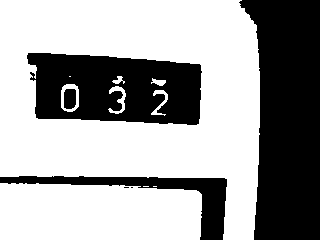
\includegraphics[scale=0.5]{otsu.png}
  \caption{Otsu算法}
  \label{fig:otsu}
\end{figure}

\subsection{连通成分筛选}

观察图\ref{fig:otsu}可得,二值化的图像黑色部分不仅包含数字边框,还包含其他几个区域,如电流表指针盘的边框和右侧的边框。这些区域需要去除,只保留数字边框。


由于这几个区域都是黑色区域,为了区分这几个区域,可以用连通成分标记算法给不同的区域赋予不同的标记。一般情况下,区域内可能有空洞或裂痕,连通成分标记可能失效。但这里的图像二值化的效果较好,区域内部不存在裂痕,适合用连通成分标记算法处理。本文选用\ref{sec:comp}节介绍的逐行扫描算法进行连通成分标记。逐行扫描算法使用并查集记录等价关系。扫描过程中算法对并查集进行大量的$\union$和$\find$操作,因此$\union$和$\find$操作的效率关系到算法的效率。

用两种策略可以优化$\find$和$\union$操作。第一种策略是\emph{按秩合并},对任意元素$x$,它的\emph{秩}定义为从该结点到其后代结点的最长路径的边数的上界,记作$rank[x]$。当用$\make(x)$创建仅包含元素$x$的集合时,$rand[x]=0$。所有$\find(x)$操作不改变$rank[x]$。进行$\union(x,y)$操作时,比较结点$x$和结点$y$的祖先的秩,如果不相等,将秩较低的根结点指向秩较高的根结点,两者的秩不增加;如果相等,则任选一个根结点指向另一个根结点,并增加新的根结点的秩。另一种策略是\emph{路径压缩}。它用于$\find(x)$操作,将其访问的所有的结点都直接指向根结点。

%用并查集使逐行扫描算法更加高效。算法第一次扫描,找到种子像素时,设定一个标号,并在并查集中创建一个只包含该标号的集合。在将标号传播到右下方的邻接点的过程中,如果发现两个不同的标号传播到同一个像素,只传播较小的标号,并将两个标号所在的集合合并。第一次扫描结束后,所有标号所在的集合均已确定。在第二次扫描时,将像素的标号改成该标号所在集合的代表标号。

连通成分标记算法的结果如图\ref{fig:candidate}所示,不同区域已经用不同的灰度区分。
\begin{figure}[h]
  \centering
  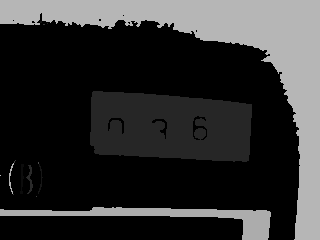
\includegraphics[scale=0.5]{candidate.png}
  \caption{连通成分}
  \label{fig:candidate}
\end{figure}


标记完各个连通成分后,下一步是从中找出数字边框。对这些连通成分进行分析。首先对连通成分进行初步分析,得到每个连通成分的基本特征,如像素数$n$和包围连通成分的最小矩形的长$L$和宽$W$等。在这些基本特征的基础上可以得到另一些特征。如长宽比$r=L/W$,面积$S=L\times R$等。再定义连通成分的区域密度为$\rho=n/S$。实验发现,数字边框对应的连通成分的各个特征具有如下范围:
\begin{equation}
  \label{eq:range}
  \begin{cases}
    8000  <  p  <  10000 \\
1.9  <  r  <  2.9 \\
0.6  <  \rho  < 0.9 
  \end{cases}
\end{equation}
因此,对每个连通成分计算这些特征值,发现落在式\eqref{eq:range}所示范围的,可以认定为数字边框。找出的数字边框如图\ref{eq:frame}所示。
\begin{figure}[h]
  \centering
  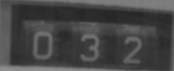
\includegraphics[scale=0.5]{frame.png}
  \caption{数字边框}
  \label{eq:frame}
\end{figure}

\subsection{倾斜校正}

因拍摄的角度问题,数字及其边框有一定的倾斜角度。因此找出数字边框后,为便于数字分割与识别,应对数字边框图像进行倾斜矫正。具体做法是先找出数字边框的上下两条横线,这两条横线的倾斜角度作为整个数字边框的倾斜角度,然后根据倾斜度旋转图像,使边框水平。

用边缘检测算子可以找出上下两条横线。由于数字边框较小,虚假的边缘对横线的倾斜角度有较大影响,边缘检测应尽量准确。为了提高边缘检测的准确度,减少虚假边缘,本文使用Canny边缘检测算子。OpenCV实现了边缘检测算子函数,但需要提供高低两个阈值。由\ref{sec:edge2d}节可知,高低阈值用于Canny算子的非最大值抑制过程,只有高于这两个阈值的边缘才得以保留。这两个阈值可以在进行仪表自动识别前确定。具体做法是用Sobel算子或Prewitt算子求出原始图像的梯度图像,由于需要保留的边缘数字边框上下两条横线,因此找出横线上较高的幅值作为高阈值,较低的幅值作为低阈值。边缘检测的结果如图\ref{fig:canny}所示。
\begin{figure}[h]
  \centering
  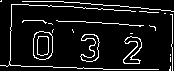
\includegraphics[scale=0.5]{canny.png}
  \caption{Canny算子}
  \label{fig:canny}
\end{figure}

边缘检测算子只能找到所有边缘点,还应从边缘点中找出上下两条横线。本文采用哈夫变换检测这些直线,将其倾斜度作为整个边框的倾斜度。在用OpenCV进行哈夫变换时,需要指定直线的参数$\theta$和$\rho$的量化间隔$\Delta\theta$和$\Delta\rho$。量化间隔太小,计算量过大,并将出现一条边缘线分裂成几条短线的情况;量化间隔太大,检测出的直线不准确。需要反复实验,找出最佳的量化间隔。实验发现,最佳的量化间隔为$\Delta\theta=2^\circ,\Delta\rho=2$。无论如何选取阈值,都无法避免边框断裂成几条直线。因此在计算直线倾斜角时,应该统计多条直线的倾斜角的平均值。求出倾斜度$\theta$后,再将边框图像绕中心按反方向旋转$\theta$角度,使整个边框处于水平位置。旋转后的图像如图\ref{fig:rotate}所示。
\begin{figure}[h]
  \centering
  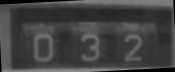
\includegraphics[scale=0.5]{rotate.png}
  \caption{旋转后的图像}
  \label{fig:rotate}
\end{figure}

\section{数字分割}

目前没有一种通用的分割方法,适用于各个领域。应该根据实际情况和领域知识,灵活地选定一种方案。

\section{数字识别}



%%% Local Variables: 
%%% mode: latex
%%% TeX-master: "thesis"
%%% End: 
